% $Id$

% Earth System Modeling Framework
% Copyright 2002-2016, University Corporation for Atmospheric Research,
% Massachusetts Institute of Technology, Geophysical Fluid Dynamics
% Laboratory, University of Michigan, National Centers for Environmental
% Prediction, Los Alamos National Laboratory, Argonne National Laboratory,
% NASA Goddard Space Flight Center.
% Licensed under the University of Illinois-NCSA License.

\documentclass[]{article}

\usepackage{epsf}
\usepackage{html}
\usepackage{times}
\usepackage{alltt}
\usepackage[T1]{fontenc}
\usepackage[dvips]{graphics,color}

\textwidth 6.5in
\textheight 8.5in
\addtolength{\oddsidemargin}{-.75in}
\newcommand{\mytitle}{Coupled Flow Demonstration}
\newcommand{\myauthors}{Jon Wolfe, Nancy Collins, Cecelia DeLuca}
\newcommand{\myversion}{Version 1.0}

% set a standard paragraph style
\setlength{\parskip}{0pt}
\setlength{\parindent}{0pt}
\setlength{\baselineskip}{11pt}
% these are temporary patches until something more
% permanent is done to the protex script.
\newlength{\oldparskip}
\newlength{\oldparindent}
\newlength{\oldbaselineskip}

\begin{document}

\bodytext{BGCOLOR=white LINK=#083194 VLINK=#21004A}

% Title page
\input{title_alldoc}

\newpage
\tableofcontents

\newpage
\setlength{\parskip}{1.5ex}

% $Id$

% Earth System Modeling Framework
% Copyright 2002-2015, University Corporation for Atmospheric Research,
% Massachusetts Institute of Technology, Geophysical Fluid Dynamics
% Laboratory, University of Michigan, National Centers for Environmental
% Prediction, Los Alamos National Laboratory, Argonne National Laboratory,
% NASA Goddard Space Flight Center.
% Licensed under the University of Illinois-NCSA License.

\section{ESMF COUPLED\_FLOW Demonstration Program}
\label{sec:demo}

\subsection{ESMF COUPLED\_FLOW Description}

The {\tt ESMF COUPLED\_FLOW} application uses the ESMF framework, including 
gridded and coupler components, Superstructure and Infrastructure. 
The application injects a tracer from one gridded
component into another, which then advects the flow.  Communication is handled through a
coupler component.  Review of this demonstration should enable the user to
understand the general structure of an ESMF application.

 
The application is comprised of two ESMF 
{\tt Gridded Components} and a {\tt Coupler Component}.  
The first {\tt Gridded Component}, {\tt FlowSolver}, solves the compressible 
time-dependent fluid flow equations.  The algorithm 
applies an explicit finite difference technique to a staggered, Arakawa C igrid 
that is Cartesian and uniform.  State variables, including density, 
pressure, viscosity and temperature, are located at cell-centers, while 
velocities are located at the north and east cell faces.  This component is initialized 
with a steady-state, one-dimensional flow.  The second {\tt Gridded 
Component}, {\tt Injector}, injects tracer fluid into the first component normal to the 
flow along 
one of the boundaries.  The injected fluid can have arbitrary velocity, 
temperature, density and duration, effectively setting some of 
the boundary conditions for the first component.  The {\tt FlowSolver} and 
{\tt Injector Components} sit on different Cartesian igrids.  The
{\tt Coupler Component} redistributes boundary condition data from 
the {\tt Injector} to the {\tt FlowSolver}.



% $Id$

\subsection{Program Organization}

The demonstration program consists of a top level Application
Driver, a top level Gridded Component, and nested within this Gridded
Component are 3 subcomponents: a Coupler Component and 2 Gridded Components.

The following diagram shows this organization.  Note that there
is no direct communication between the subcomponents; all
interactions are mediated by the top level Gridded Component.

Each component communicates via initialize, run, and finalize
subroutine calls.  These go through the ESMF library where
they are checked for validity, default values are supplied,
and only those components involved in the computation are
invoked.

% the bpht says we prefer the bottom of a page, then separate page,
% then here, then top last.

\begin{figure}[bpht]
\caption[Components]{Structure of the demonstration program.}
\label{fig:democomps}
\begin{center}
\scalebox{0.70}{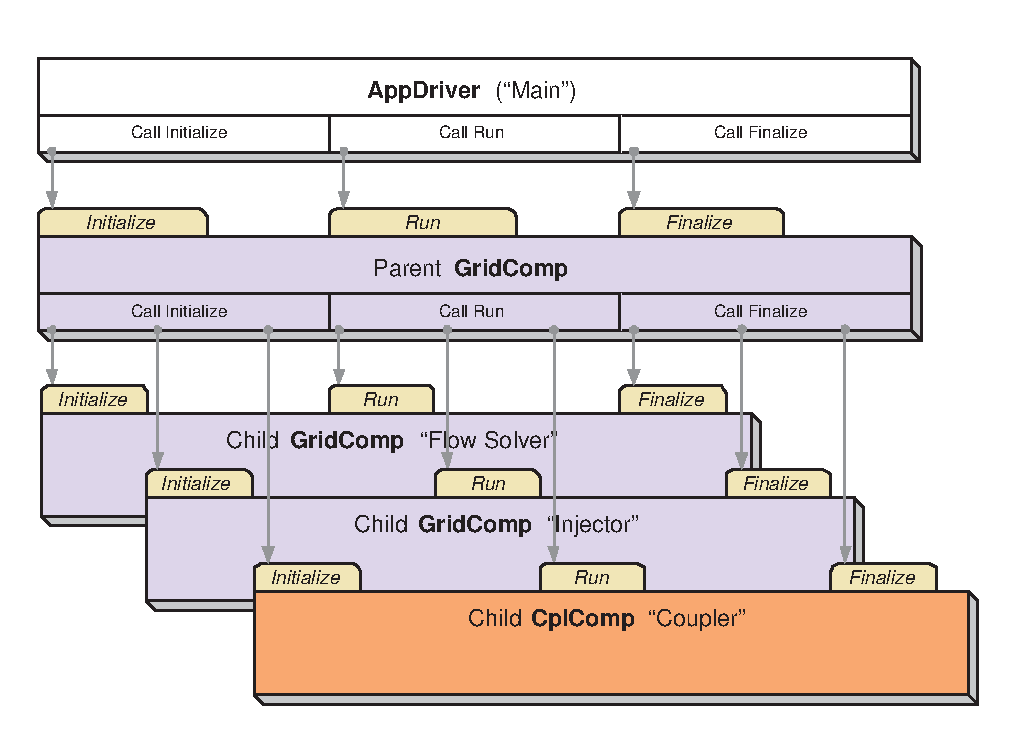
\includegraphics{flow_struct.eps}}
\end{center}
\end{figure}




\section{ESMF COUPLED\_FLOW Demonstration Code Details}

\input{CoupledFlowApp_fapi}

\input{CoupledFlowDemo_fapi}

\input{FlowSolverMod_fapi}

\input{FlowArraysMod_fapi}

\input{CouplerMod_fapi}

\input{InjectorMod_fapi}

\input{InjectArraysMod_fapi}

\input{FlowUtilMod_fapi}

%\bibliography{ESMF} 
\bibliographystyle{plain}
\addcontentsline{toc}{section}{Bibliography}

\end{document}
